\documentclass[12pt,a4paper]{article}
\usepackage[spanish,es-tabla]{babel}

\usepackage[utf8]{inputenc} % Escribir con acentos, ~n...
\usepackage{eurosym} % s´ımbolo del euro
\newcommand{\horrule}[1]{\rule{\linewidth}{#1}} % Create horizontal rule command with 1 argument of height
\usepackage{listings}             % Incluye el paquete listing
\usepackage[cache=false]{minted}
\usepackage{graphics,graphicx, float} %para incluir imágenes y colocarlas
\usepackage{hyperref}
\hypersetup{
	colorlinks,
	citecolor=black,
	filecolor=black,
	linkcolor=black,
	urlcolor=black
}
\usepackage{multirow}
\usepackage{array}
\usepackage{diagbox}

\title{
\normalfont \normalsize 
\textsc{{\bf Aprendizaje Automático (2018-2019)} \\ Grado en Ingeniería Informática \\ Universidad de Granada} \\ [25pt] % Your university, school and/or department name(s)
\horrule{0.5pt} \\[0.4cm] % Thin top horizontal rule
\huge Práctica 1 \\ % The assignment title
\horrule{2pt} \\[0.5cm] % Thick bottom horizontal rule

\includegraphics{images/logo.png}	
}

\author{Antonio Jesús Heredia Castillo} % Nombre y apellidos

\date{\normalsize\today} % Incluye la fecha actual

%----------------------------------------------------------------------------------------
% DOCUMENTO
%----------------------------------------------------------------------------------------

\begin{document}

\maketitle % Muestra el Título
\newpage %inserta un salto de página
\tableofcontents % para generar el índice de contenidos
\listoffigures
\listoftables
\newpage

\section{Gradiente descendente}
\subsection{Implementar el algoritmo de gradiente descendente}
He querido implementar el algoritmo del gradiente descendente de la forma mas general que he podido. Para ello, he creado una función que lo calcula. Esta función recibe  los siguientes parámetros:
\begin{itemize}
	\item lr (float): Tasa de aprendizaje
	\item punto (array[x,y]): Punto desde el cual se quiere aplicar el algoritmo
	\item función (float): Función a la que se le quiere aplicar el gradiente descendente
	\item iteraciones (int): Numero máximo de iteraciones que aplicara el algoritmo
\end{itemize}
Esta subrutina se encarga de hacer las derivadas parciales de la función y de calcular de forma iterativa el punto mínimo de la función. En esta primera versión del algoritmo, la única condición de parada va a ser el numero de iteraciones que le pasa el usuario. Podemos ver el código del algoritmo aquí.
\begin{minted}[mathescape,
	frame=lines,
	framesep=2mm]{python}
_iter = 0 #Contador de iteraciones
_dx = sp.diff(funcion, x) #Derivadas parciales
_dy = sp.diff(funcion, y)
#Lambdifyco las derivadas parciales para calcular mas rapido el valor
_lam_dx = sp.lambdify((x,y),_dx) 
_lam_dy = sp.lambdify((x,y),_dy)
while True:
	#creo una copia del punto, para que a la hora de evuluar el x, 
	#no lo pierda para y
	_punto_copia = np.copy(_punto)
	#si hay mas iteraicones de las que yo quiero paro
	if _iter > _iteraciones:
		break
	#calculo el gradiente
	_punto[0] = _punto[0]-_lr*_lam_dx(_punto_copia[0],_punto_copia[1])
	_punto[1] = _punto[1]-_lr*_lam_dy(_punto_copia[0],_punto_copia[1])
	_iter =_iter+1
return _punto   
\end{minted}

\subsection{Considerar la Función \(  E(u, v) = (u^2e^v - 2v^2e^{-u})^2\). Usar gradiente descendente para encontrar un mínimo de esta función, comenzando desde el punto \((u, v) = (1, 1)\) y usando una tasa de aprendizaje \(\eta = 0,01\).}
\subsubsection{Calcular analíticamente y mostrar la expresión del gradiente de la función \(E(u, v)\)}
Lo primero que tenemos que saber es que para calcular el gradiente, necesitamos las derivadas parciales de \(E(u,v)\). \\
La derivada respecto de \(u\) seria: 

\begin{equation}
\frac{\partial E(u,v)}
{\partial u} = 2\left(u^2e^v-2v^2e^{-u}\right)\left(2e^vu+2v^2e^{-u}\right)
\end{equation}
La derivada respecto de \(v\) seria: 
\begin{equation}
\frac{\partial E(u,v)}
{\partial v} = 2\left(u^2e^v-2v^2e^{-u}\right)\left(u^2e^v-4e^{-u}v\right)
\end{equation}
El vector gradiente seria las dos derivadas parciales en el punto  $(u, v) = (1, 1)$.
\begin{equation}
\nabla E(1,1) = (E_u(1,1),E_v(1,1)) = (12.236771,2.4717385)
\end{equation}
Ahora con las derivadas, ya podemos obtener el gradiente. Los nuevos valores de \(u\) y \(v\) serán:
\begin{equation}
u' = u - 2\eta\left(u^2e^v-2v^2e^{-u}\right)\left(2e^vu+2v^2e^{-u}\right)
\end{equation}

\begin{equation}
v' = v - 2\eta\left(u^2e^v-2v^2e^{-u}\right)\left(u^2e^v-4e^{-u}v\right)
\end{equation}

Por lo tanto para el punto $(u, v) = (1, 1)$ el valor del gradiente seria:
\begin{equation}
u' = 1 - 2*0.01\left(1^2e^1-21^2e^{-1}\right)\left(2e^1+21^2e^{-1}\right) = 0.75526458
\end{equation}

\begin{equation}
v' = 1 - 2*0.01\left(1^2e^1-21^2e^{-1}\right)\left(1^2e^1-4e^{-1}1\right) = 0.95056523
\end{equation}
\subsubsection{¿Cuántas iteraciones tarda el algoritmo en obtener por primera vez un valor de \(E(u, v)\) inferior a \(10^{-14}\) . (Usar flotantes de 64 bits)}
Para realizar este ejercicio, solo he metido una condición de parada en el algoritmo. La condición de parada en este caso es que el valor de evaluar \(E(u,v)\) en un determinada iteración sea \(E(u,v)<10^{-14}\)

\begin{minted}[mathescape,
frame=lines,
framesep=2mm]{python} 
if _iter > _iteraciones or 
   _lam_f(_punto_copia[0],_punto_copia[1]) < np.float64(10**-14):
	print ("La funcion ha acabado a las " 
	+ str(_iter) + " iteraciones")
	break
\end{minted}
En este caso el numero de iteraciones necesarias ha sido \textbf{33}, como se puede ver en la Figura\ref{figura1}.

\begin{figure}[H]  %con el [H] le obligamos a situar aquí la figura
\centering
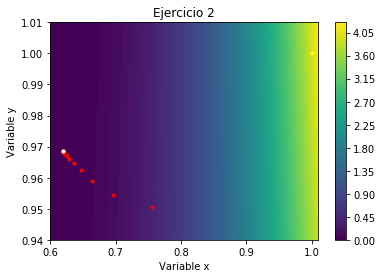
\includegraphics{images/primerDescensoGradiente.png}  %el parámetro scale permite agrandar o achicar la imagen. En el nombre de archivo puede especificar directorios
\caption{Representación de como avanza el gradiente en la función \(E(u,v)\). Punto en amarillo inicio y punto final en blanco.}
\label{figura1}
\end{figure}

\subsubsection{¿En qué coordenadas \((u, v)\) se alcanzó por primera vez un valor igual o menor a \(10^{-14}\) en el apartado anterior.}
Como el algoritmo del gradiente me devuelve el punto en el que acaba, lo único que tengo que hacer es mostrarlo por pantalla. En este caso el punto en el que se alcanza \(10^{-14}\) es \textbf{\((0.61920768,0.96844827)\)}.

\subsection{Considerar ahora la función \(  f(x,y)=x^2+2y^2+2\sin(2\pi x)\sin(2\pi y)\)}
\subsubsection{Usar gradiente descendente para minimizar esta función. Usar como punto inicial \((x_{0}=0.1, y_{0}=0.1)\), (tasa de aprendizaje \(\eta=0,01\) y un máximo de 50 iteraciones. Generar un gráfico de cómo desciende el valor de la función con las iteraciones. Repetir el experimento pero usando \(\eta=0.11\), comentar las diferencias y su dependencia de \(\eta\).}
Usando un \(\eta=0.01\), podemos gráficamente Figura  \ref{figura2} como el gradiente desciende de forma adecuada. En este caso acaba en una altura de \(-1.8200785415471563\)

\begin{figure}[H]  %con el [H] le obligamos a situar aquí la figura
	\centering
	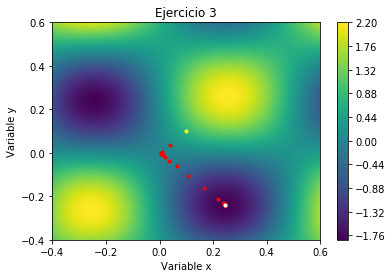
\includegraphics{images/segundoDescensoGradiente1.png}  
	\caption{Gradiente de la función \(F(u,v)\) con   \((x_{0}=0.1, y_{0}=0.1)\) y \(\eta=0.01\). Punto en amarillo inicio y punto final en blanco.}
	\label{figura2}
\end{figure}
En cambio cuando usamos \(\eta=0.1\) , podemos ver (Figura  \ref{figura3}) como no funciona bien. En este caso acaba en una altura de \(2.5007003656467446\), que es incluso mas alto que desde donde empezamos (\(0.7209830056250534\)).
\begin{figure}[H]  %con el [H] le obligamos a situar aquí la figura
	\centering
	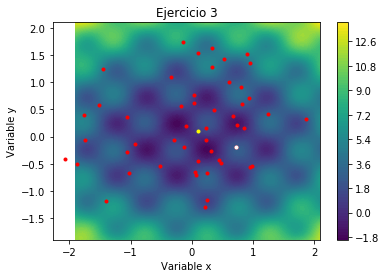
\includegraphics{images/segundoDescensoGradiente2.png}  
	\caption{Gradiente de la función \(F(u,v)\) con   \((x_{0}=0.1, y_{0}=0.1)\) y \(\eta=0.1\). Punto en amarillo inicio y punto final en blanco.}
	\label{figura3}
\end{figure}
Las diferencias entre usar un \(\eta\) muy grande o uno adecuado es clara viendo las imágenes, con \(\eta\) adecuado se encuentra ``rápidamente'' el mínimo. Con el \(\eta\) muy grande, el algoritmo da saltos muy grandes y por lo tanto no llega a encontrar el mínimo debido a que de una iteración a otra lo excede y empieza a rebotar sin encontrar nada.
\subsubsection{Obtener el valor mínimo y los valores de las variables \((x, y)\) en donde se alcanzan cuando el punto de inicio se fija: \((0,1, 0,1), (1, 1),(-0,5, -0,5),(-1, -1)\). Generar una tabla con los valores obtenidos}
Los datos obtenidos podemos verlos en la Tabla \ref{tab:puntos}. En este caso, no he dejado el calculo de todos los puntos en el código para no sobrecargar la salida por pantalla con datos y que el tiempo de ejecución no fuera muy alto. El campo ``valor'' indica la altura que alcanza la función en el punto \((x,y)\).
\begin{table}[H]

	\caption {La altura minima conseguida en los diferentes puntos con GD} \label{tab:puntos} 
	   
	\begin{tabular}{|l|r|r|r|r|}
		\hline
		\backslashbox{Valor final}{Punto} &  \((0.1 , 0.1)\) & \((1 , 1)\) & \((-0.5 , -0.5)\) & \((-1 , -1)\)\\
		\hline
		x & 0.24380497 & 1.2180703  & -0.73137746  & -1.2180703\\
		\hline
		y & -0.23792582 & 0.71281195 & -0.23785536 & -0.71281195\\
		\hline
		Valor mínimo & -1.82007854 & 0.59326937 & -1.33248106 & 0.59326937\\
		\hline
	\end{tabular}
\end{table}
\subsubsection{¿Cuál sería su conclusión sobre la verdadera dificultad de encontrar el mínimo	global de una función arbitraria?}
Teniendo en cuenta los datos obtenidos en los apartados anteriores y como afecta tanto la tasa de aprendizaje como el punto donde se inicia el algoritmo. Llego a la conclusión que la verdadera dificultad radica en la elección de estos dos parámetros. Por ejemplo al elegir un ``mal'' punto de inicio puede no encontrar el punto mínimo absoluto de la función, si no un punto mínimo relativo a la posición desde donde ha iniciado. \\\\
Elegir una tasa de aprendizaje que no sea adecuada también nos va a dar bastantes problemas. Esto se debe a que si es muy grande, el algoritmo nunca va a llegar a converger debido a que va a ir rebotando de un lado al otro del mínimo, pero sin llegar a acercarse nunca. Si lo elegimos muy pequeño, el algoritmo daría pasos muy pequeños y tardaría demasiado en llegar al mínimo.\\\\
Por lo tanto desde mi punto de vista una vez que tienes todos los algoritmos implementados, la dificultad radica en elegir buenos valores para conseguir que nuestro algoritmo funcione de forma adecuada.\textbf{}
\section{Regresión lineal}
\subsection{Estimar un modelo de regresión lineal a partir de los datos proporcionados usando tanto el algoritmo de la pseudoinversa como  SGD}
Para la implementación del SGD, he añadido un pequeño cambio al algoritmo original. Lo primero que he realizado es añadir una condición de parada por numero de iteraciones. Por si el epsilon que utilizo es muy pequeño y el algoritmo no consigue ``converger''. \\Otro cambio que he realizado, muy simple pero efectivo, es que en caso de que no consiga converger y pare por numero de iteraciones, lo que realizo es llevar una copia de la $w$ con menor $E_{in}$ que he obtenido y esos son los pesos y el error que devolveré. Asegurando así obtener el mejor modelo que he conseguido calcular, pero dejando la posibilidad de salir de mínimos locales.
\subsubsection{ Pintar las soluciones obtenidas junto con los datos usados en el ajuste.}
La configuración que he usado para realizar el SGD ha sido la siguiente:
\begin{itemize}
	\item $\eta=0.01$.
	\item Tamaño del minibatch: 64.
	\item Nº de iteraciones: 1000.
\end{itemize}
Los pesos que he conseguido con esta configuración de SGD y la pseudoinversa los podemos ver en la Tabla \ref{tab:pesos}
	
\begin{table}[H]
	\centering
	\caption {Los pesos conseguido con la pseudoinversa y con SGD} \label{tab:pesos} 
	
	\begin{tabular}{|l|r|r|r|}
		\hline
		\backslashbox{Método}{Pesos} & $w_0$ & $w_1$ & $w_2$\\ 
		\hline
		Pseudoinversa & -1.11588 & -1.2486  &-0.497532 \\
		\hline
		SGD & -1.24421 & -0.180105 & -0.458887\\
		\hline
	\end{tabular}
\end{table}

Podemos ver los hiperplanos que conseguimos con estos pesos en la Figura \ref{pic:hiperplanos}
\begin{figure}[H]  %con el [H] le obligamos a situar aquí la figura
	\centering
	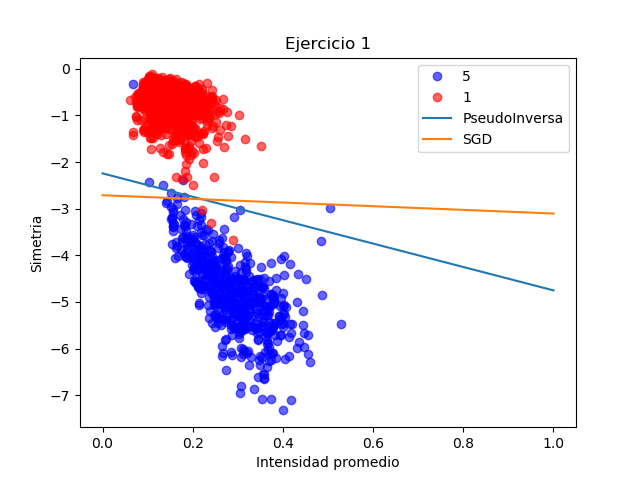
\includegraphics{images/hiperplanosEjercicio1.png}  %el parámetro scale permite agrandar o achicar la imagen. En el nombre de archivo puede especificar directorios
	\caption{Representación de los hiperplanos que conseguimos con la pseudoinversa y con SGD junto a los datos de entrenamiento.}
	\label{pic:hiperplanos}
\end{figure}
\subsubsection{Valorad la bondad del resultado usando $E_{in}$ y $E_{out}$}

Los errores que obtenemos con ambos modelos son los que podemos ver en la Tabla \ref{tab:errores}
	
\begin{table}[H]
	\centering
	\caption {Errores obtenidos con la pseudoinversa y con SGD} \label{tab:errores} 
	
	\begin{tabular}{|l|r|r|}
		\hline
		\backslashbox{Método}{Error} & $E_{in}$ & $E_{out}$\\ 
		\hline
		Pseudoinversa & 0.07918658628900402 & 0.13095383720052586 \\
		\hline
		SGD & 0.08164527370294046 & 0.1351534264237533 \\
		\hline
	\end{tabular}
\end{table}
Viendo los datos del error, podemos observar que los datos de error no son tan diferentes en los datos de entrenamiento. Pero en cambio en los datos de test, si que son mas grande para ambos, siendo aun mayores en el SGD que en la pseudoinversa.
\subsection{En este apartado exploramos como se transforman los errores $E_{in}$  y $E_{out}$ cuando aumentamos la complejidad del modelo lineal usado.}
Ahora hacemos uso de la función $simula_unif (N, 2, size)$ que nos devuelve $N$ coordenadas 2D de puntos uniformemente maestreados dentro del cuadrado definido por $[-size, size] × [-size, size]$
\subsubsection{Generar una muestra de entrenamiento de N = 1000 puntos en el cuadrado $X=[-1, 1] × [-1, 1]$. Pintar el mapa de puntos 2D.}
Genero los puntos y los muestro en la Figura \ref{pic:puntos}

\begin{figure}[H]  %con el [H] le obligamos a situar aquí la figura
	
	\centering
	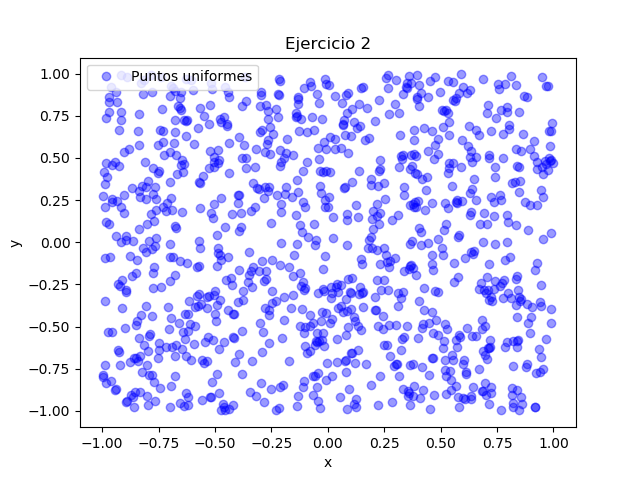
\includegraphics[width=0.7\textheight]{images/puntosEjercicio2.png}  %el parámetro scale permite agrandar o achicar la imagen. En el nombre de archivo puede especificar directorios
	\caption{Representación de los puntos.}
	\label{pic:puntos}
\end{figure}

\subsubsection{Consideremos la función $f(x_1,x_2) = sign((x_1-0,2)^2 + x^{2}_2 - 0,6)$ que usaremos para asignar una etiqueta a cada punto de la muestra anterior. Introducimos 	ruido sobre las etiquetas cambiando aleatoriamente el signo de un $10\%$ de las mismas. Pintar el mapa de etiquetas obtenido.}
Una vez etiquetados los puntos y añadido el ruido obtenemos la Figura \ref{pic:ruido}
\begin{figure}[H]  %con el [H] le obligamos a situar aquí la figura
	
	\centering
	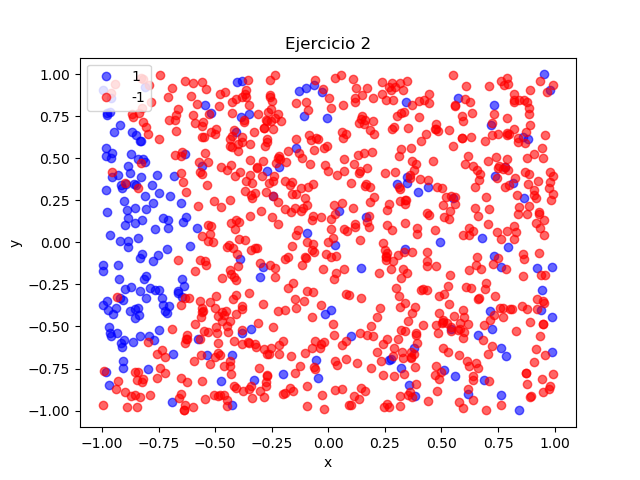
\includegraphics[width=0.7\textheight]{images/puntosConRuido.png}  %el parámetro scale permite agrandar o achicar la imagen. En el nombre de archivo puede especificar directorios
	\caption{Representación de los puntos etiquetados.}
	\label{pic:ruido}
\end{figure}
\subsubsection{Usando como vector de características (1, x 1 , x 2 ) ajustar un modelo de regresión 	lineal al conjunto de datos generado y estimar los pesos w. Estimar el error de 	ajuste E in usando Gradiente Descendente Estocástico (SGD).}
La configuración que he usado para realizar el SGD ha sido la siguiente:
\begin{itemize}
	\item $\eta=0.01$.
	\item Tamaño del minibatch: 16.
	\item Nº de iteraciones: 150. 
\end{itemize}
He elegido esta configuración con tan pocas iteraciones ya que en el siguiente apartado deberemos ejecutarla 1000 veces. Entonces para que se obtengan datos adecuados y en un tiempo razonable, he elegido esta configuración.\\
El $E_{in}$ que he obtenido es de $0.6680103340441726$ y el vector de pesos es el siguiente: $w = [-0.57499258, -0.30563394, -0.01233472]$
\subsubsection{Ejecutar todo el experimento definido 1000 veces (generamos 1000	muestras diferentes) y calcular tanto $E_{in}$ como $E_{out}$ (generaremos 1000 datos para cada test)}
El valor medio para el $E_{in}$ en las 1000 iteraciones es de $0.6493599621736924$.
El valor medio para el $E_{out}$ en las 1000 iteraciones es de $0.5267351175425848$.

\subsubsection{Valore que tan bueno considera que es el ajuste con este modelo lineal a la vista	de los valores medios obtenidos de $E_{out}$ y $E_{in}$}
Podemos ver que el $E_{out}$ es menor, esto se debe a que los test que he utilizado no tenían ningún ``ruido'' y por lo tanto, en media, se ajusta mejor. De una iteración a hacer la media con 1000 el $E_{in}$ no tiene un cambio tan acuciado.\\ Podemos ver que esta vez el ajuste no es tan bueno como en casos anteriores. Esto se debe a que la función que podría ajustar nuestros datos, no es lineal, como la que realizamos ahora, si no que debería usar alguna función que tuviera alguna curva.
\end{document}